The process that our experiment undertook was iterative. Obstacles in the analysis showed the need to develop tools that help us to make the process less cumbersome. In the same way that in the previous chapter we explored the flow of ideas that led to our pipeline design, here we will explain how data shaped our experimental process.\\

To have a complete picture of how does our approach compares with techniques from classical computer vision, we trained other models to test their performance against our novel approach.\\

\section{Exploratory analysis}

Drone images from three different towns in the state of Oaxaca where obtained from CENAPRED. During the week following the Chiapas earthquake of September 7, 2018, several drones took these pictures. We received 727 images from Santa Maria Xadani, 1872 from Union Hidalgo, and 1134 from Juchitan of Zaragoza.\\

As we can see in the following figures, drones fly in a regular pattern forming a lattice of points. It is natural to think that given the spatial distribution, that the images distribute among clusters, in other words, there exists a certain degree of similarity. We wanted to show that this clustering translates to the space of information that the images contain. To do this, we used a usual technique to our set of images.\\

\subsection{T-distributed stochastic neighbor embedding}

In the interest of being able to represent the images in a two-dimensional structure, we used a technique known as t-distributed stochastic neighbor embedding (t-SNE) analysis. It was proposed by Laurens van der Maaten \cite{t-sne}, as an alternative to traditional methods that were difficult to optimize. It usually captures the underlying structure of a set of images, and it is useful when the data lies in different, but low dimensional manifolds.\\

In our case we expected the images of the different towns to cluster in this low dimensional representation. We thought that pictures taken under in the same town would be closer than the ones taken in a different setting because of the light conditions during the exposure tend to have less variance among similar times and places. To this end, the information from the pixels of each image was flattened into a vector comprising the means and standard deviations. This simple dimensionality reduction technique was used to embed the images into a lower dimensional space. As we expected, images form natural clusters depending on the town that they depict. Our result is shown in Figure \cite{fig:tsne}.\\

The outcome obtained after applying t-SNE supported our proposed methodology of using images from one town and try to predict on others. The application detailed in the previous chapter was used to crop and classify 100 square patches from the images in each of the towns. Each piece was 327 x 327 pixels, and a tag was assigned manually by the author in each of them.\\


\begin{figure}[t]
  \begin{center}
    \subfigure{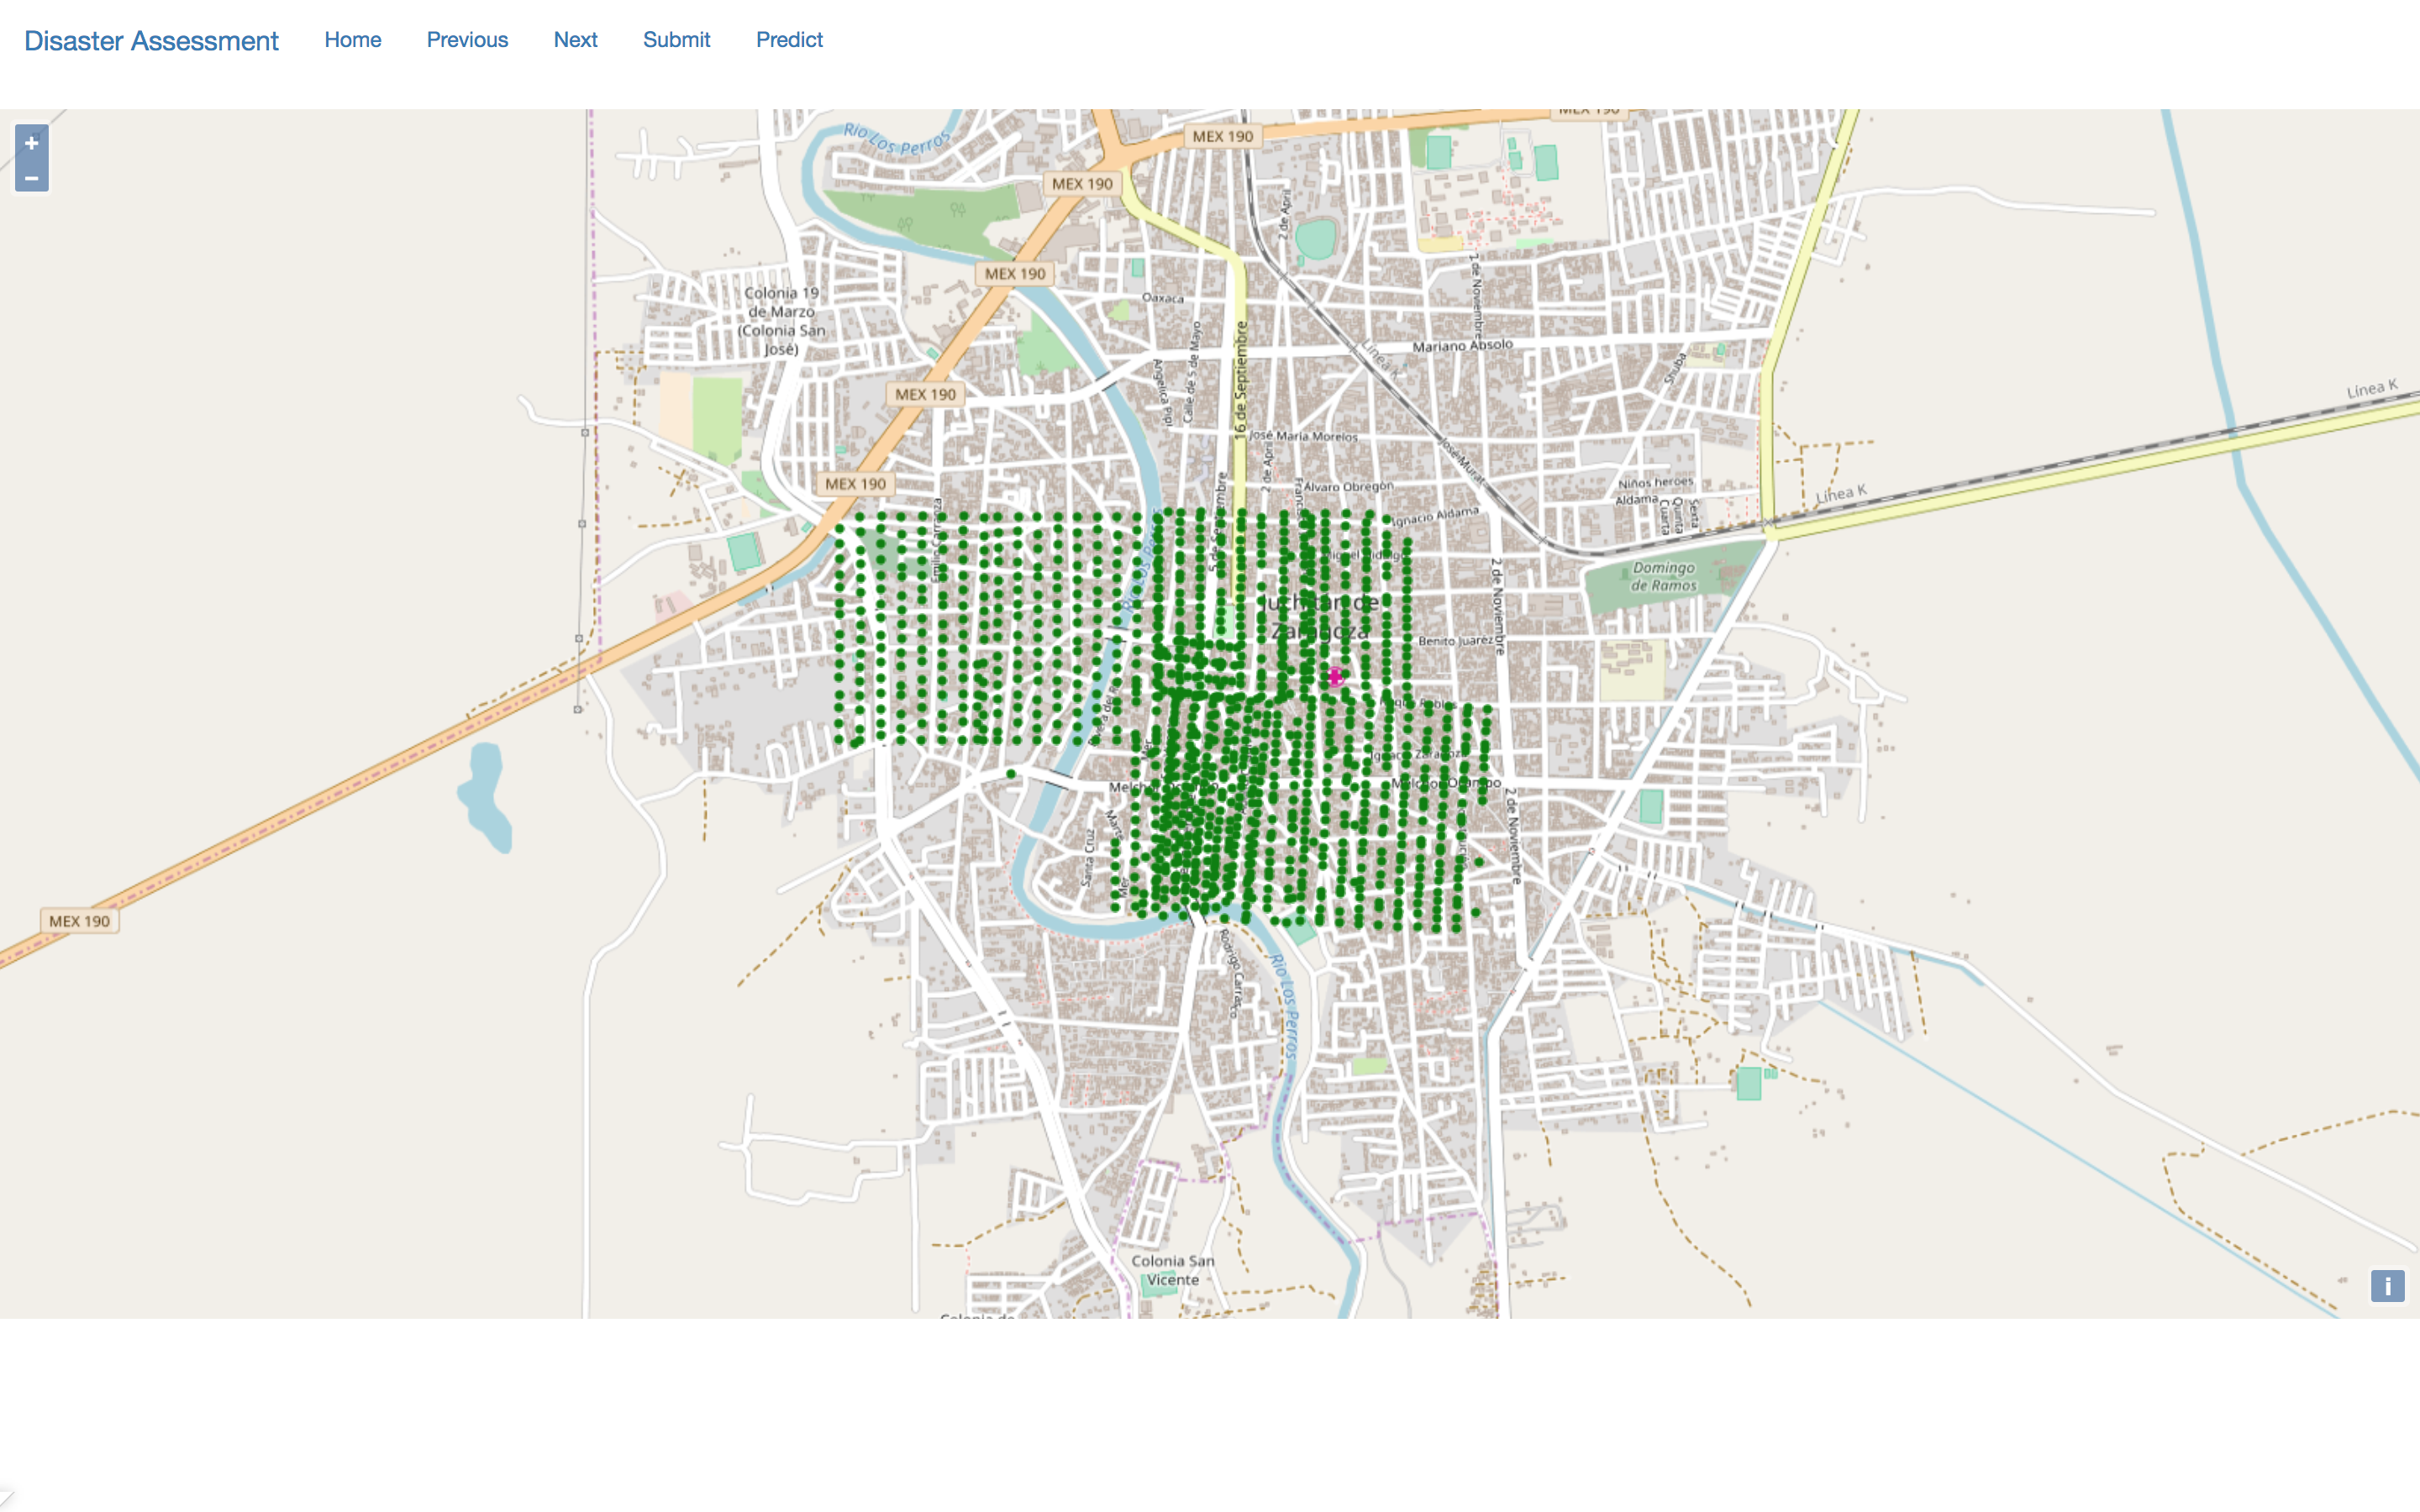
\includegraphics[width=4.25in]{images/juchitan.png}}
    \subfigure{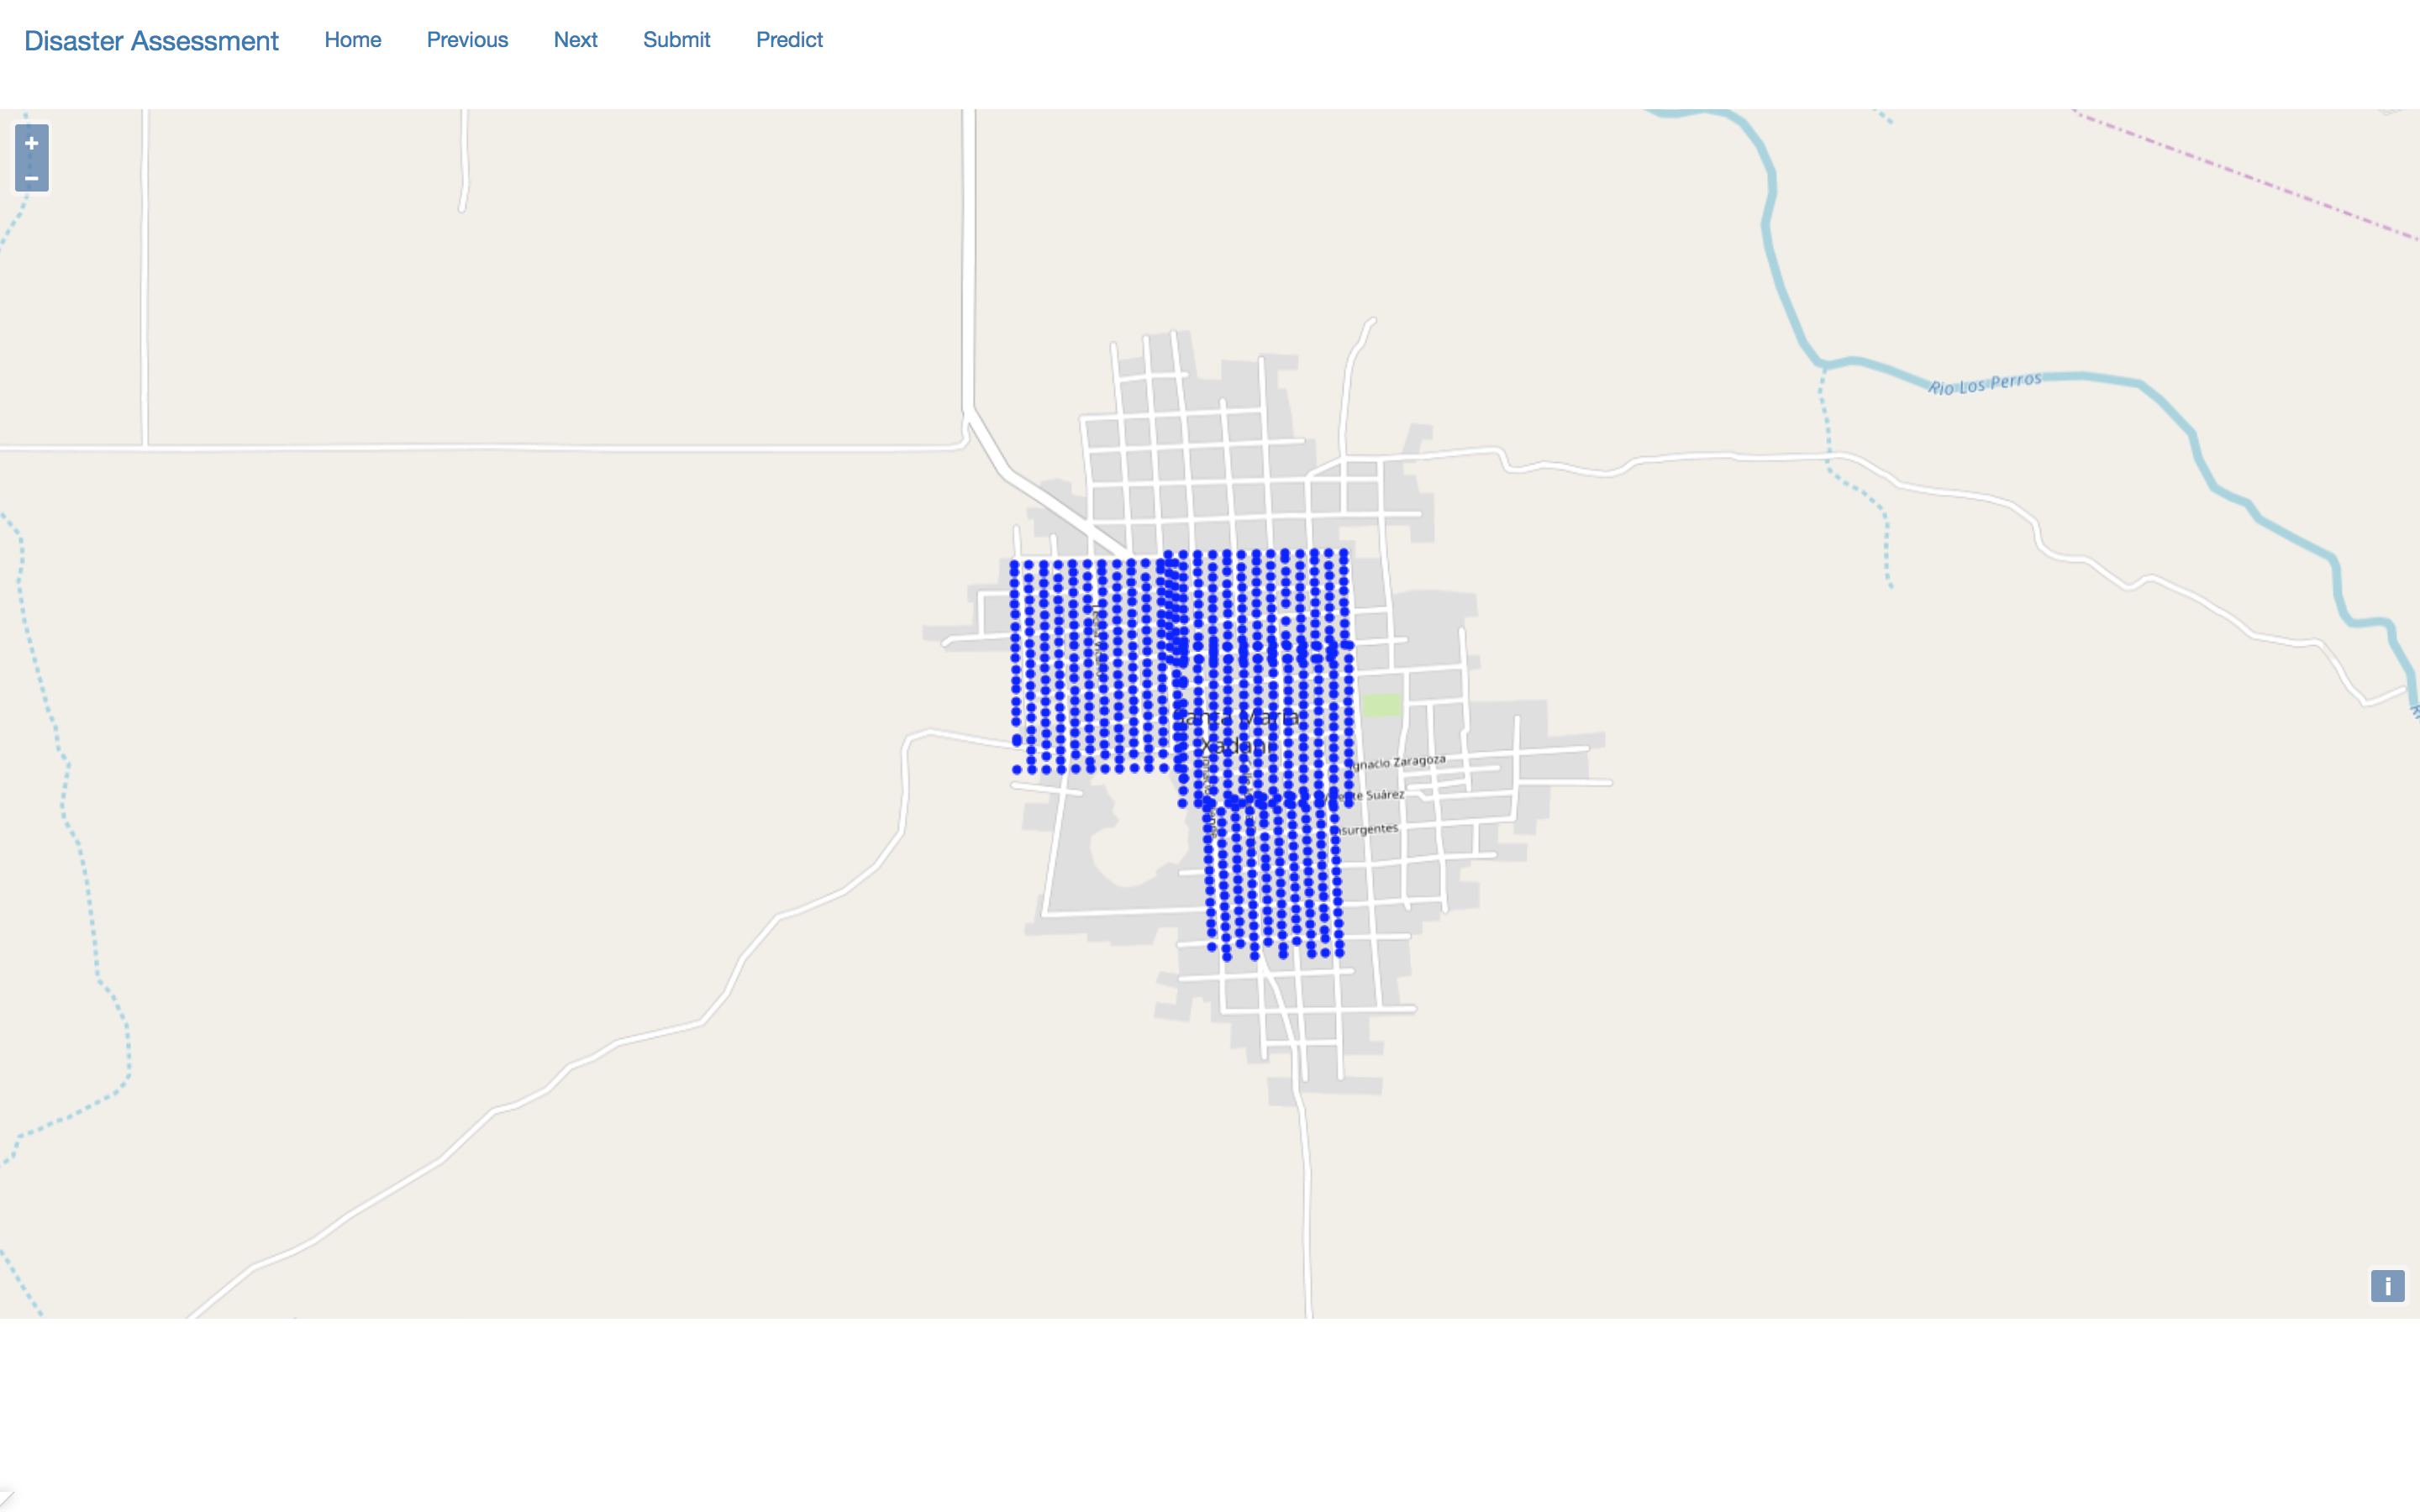
\includegraphics[width=4.25in]{images/xadani.png}}
    \subfigure{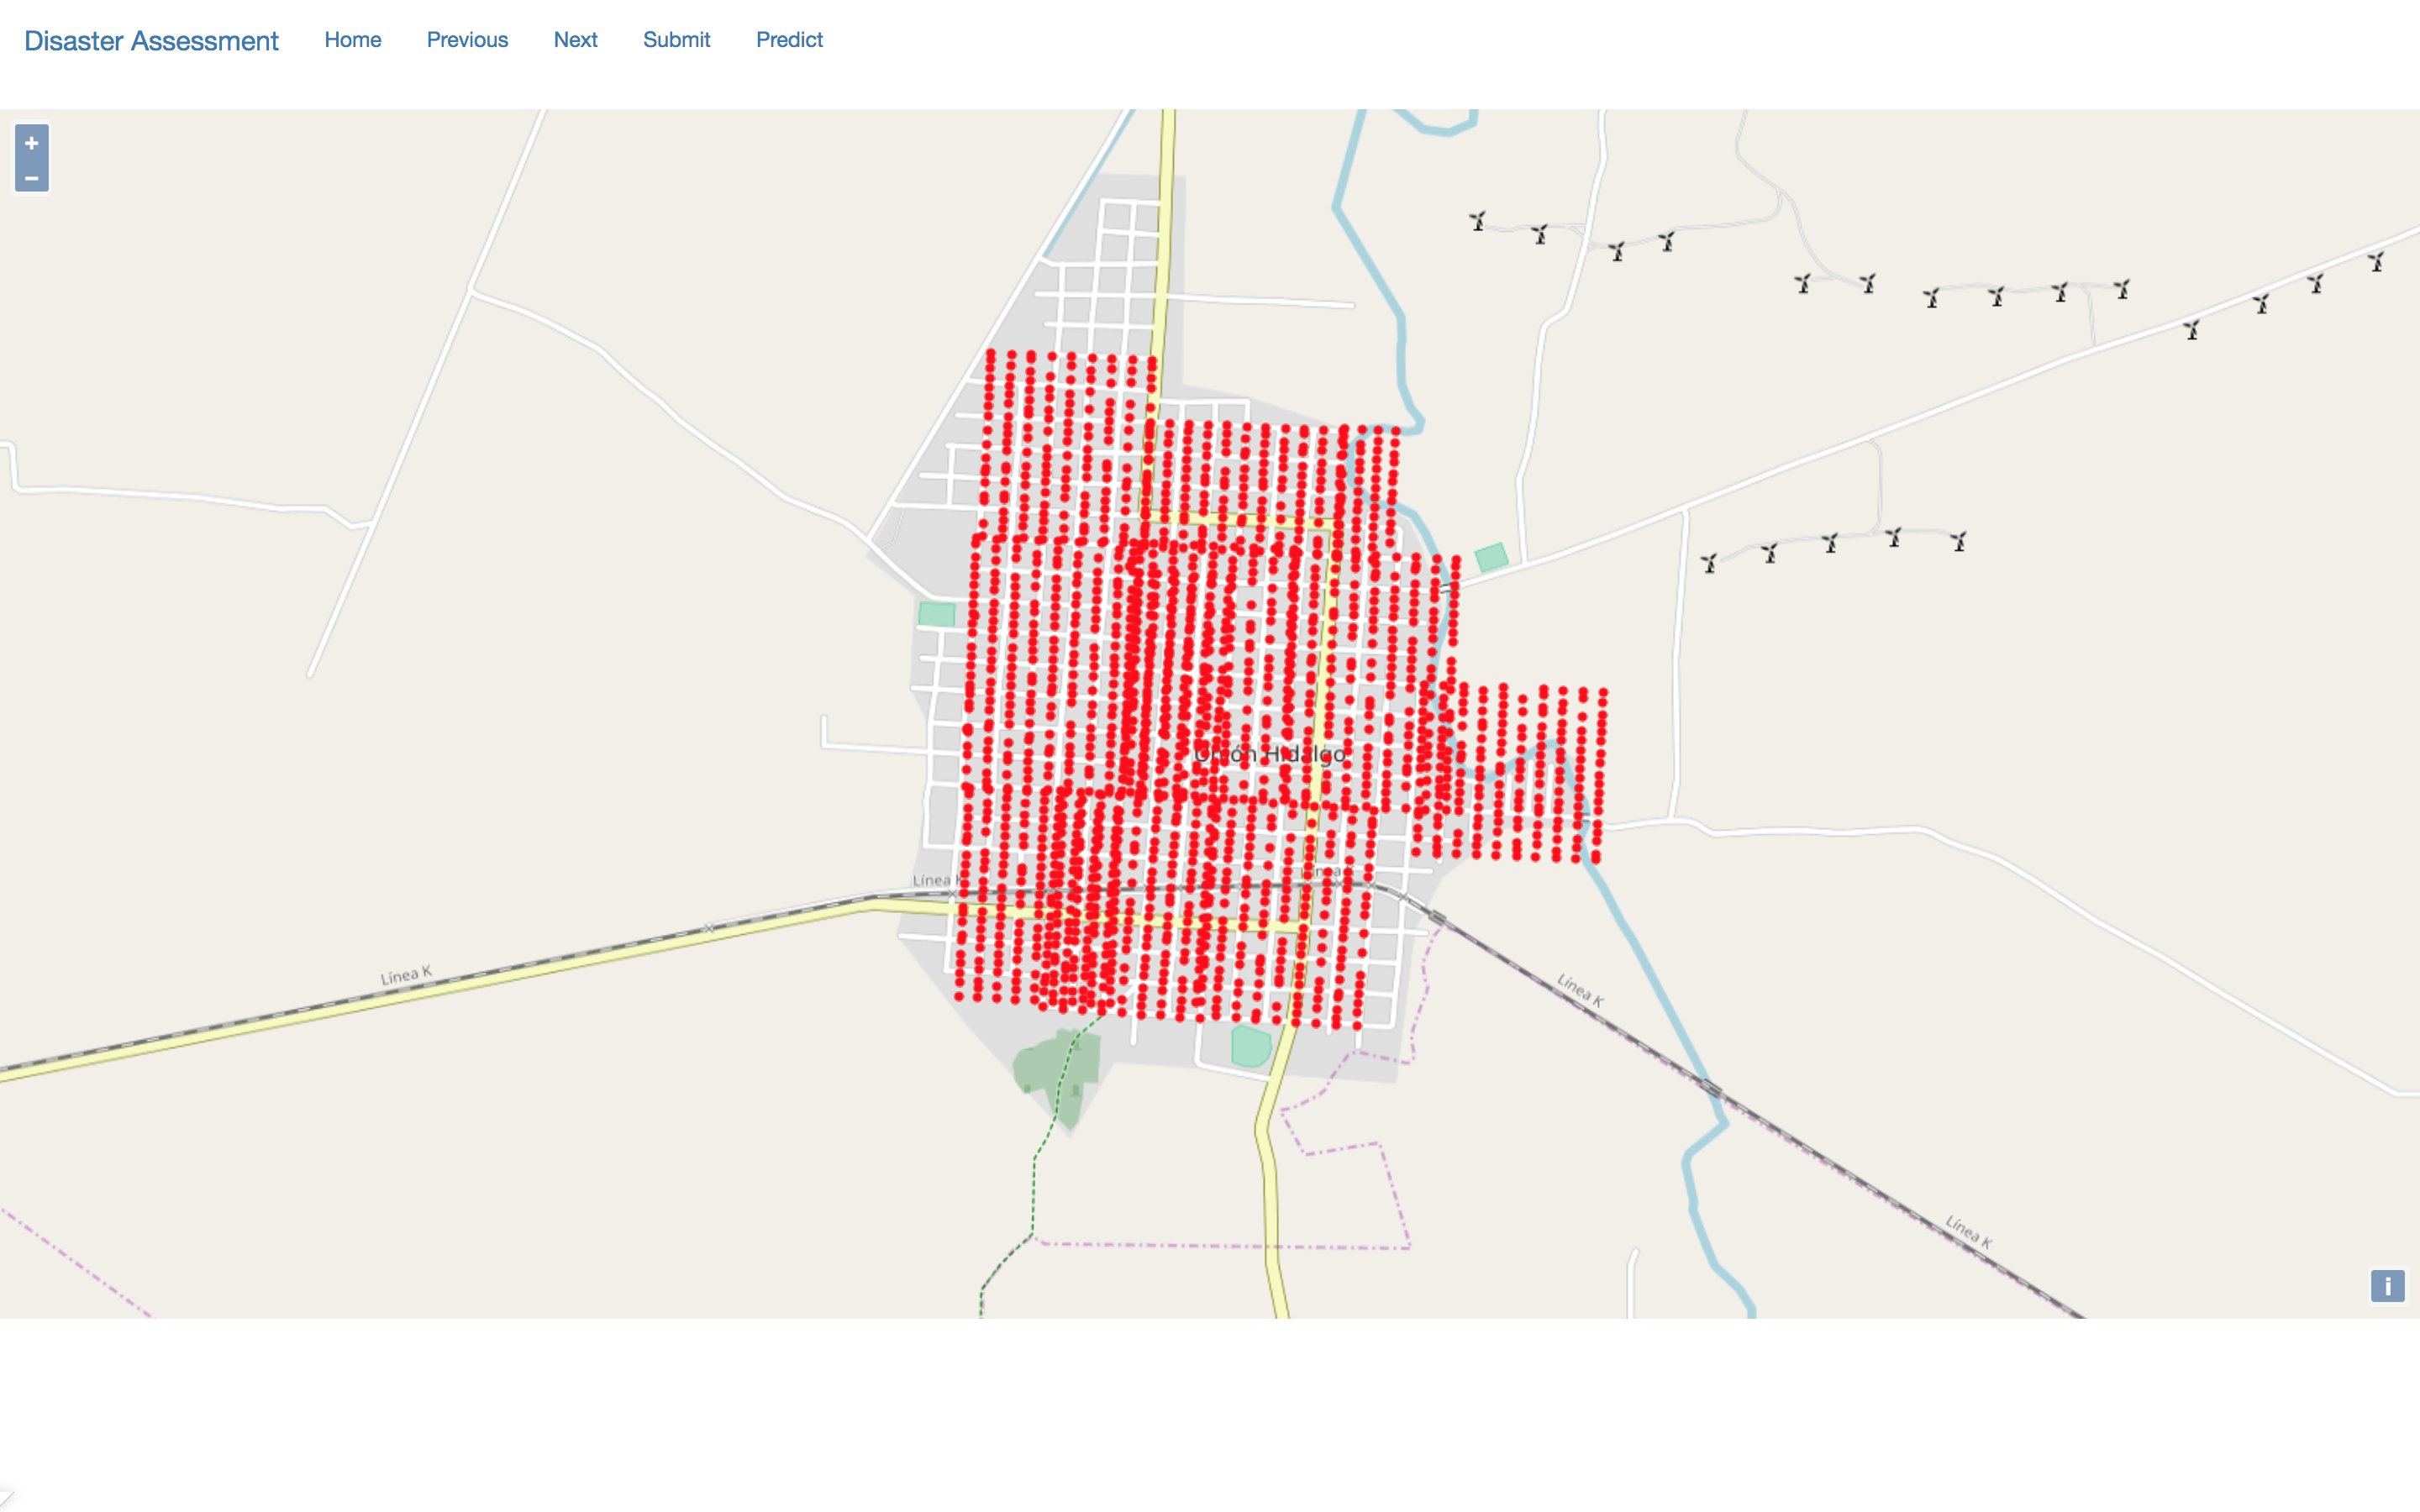
\includegraphics[width=4.25in]{images/union.png}}
  \end{center}
  \caption{Geographical location of the pictures. From top to bottom we have Juchitan de Zaragoza, Santa Maria Xadani, and Union Hidalgo.}
  \label {fig:tsne}
\end{figure}





\begin{figure}[h]
  \begin{center}
    \subfigure{\label{fig:tsne}\fbox{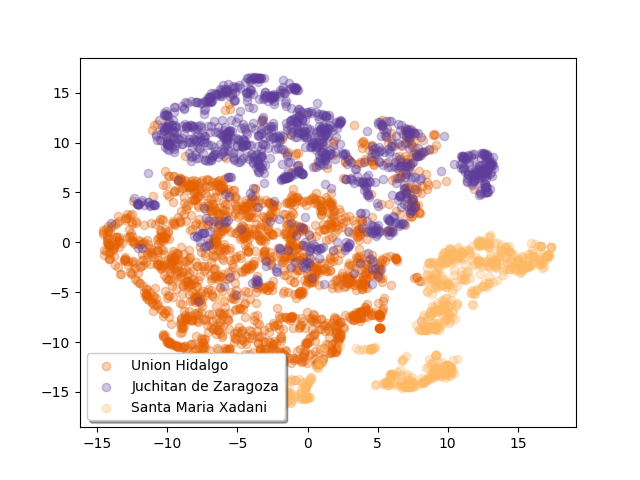
\includegraphics[width=1\textwidth]{images/t-sne.png}}}
  \end{center}
\end{figure}


\section{Model validation}

We want to train a model to be a faithful representation of the phenomena that we study, but ¿How do we know that this description is correct? We need to validate the relationship between the outcome of the model and the data that we have at hand. This process is complicated. Validation must be carefully crafted to obtain valid results.\\

Even though deep learning has allowed us to do a giant leap forward on the performance of several tasks, and contrary to what some researchers claim \cite{DBLP:journals/corr/KaiserGSVPJU17}, there exists no universal model. A good model would be able to be performant in very different settings, but it won't be able to handle every situation. We need our model to be robust, but we can not expect it to be perfect. Being aware of the limitations intrinsic to the model is the best way to alleviate possible mistakes. Although it sometimes seems the case, deep learning is not a magic box, it learns from the data that we supply. If the model is biased, in all likelihood, it means that our training set is biased.\\

To have an efficient algorithm we need it to be performant with places and images it has never seen before. A classic approach would be to divide the dataset into two parts; training and testing sets, the model is trained with the former, and then tested against the latter. This method is not used in practice because data is usually scarce and we would like to take the most of it. A better option is $n-fold$ crossed-validation in which we repeat a similar $n$ times and average the outcomes. This process makes more likely to train the model with every data point and average errors that may appear by chance. However, $n-fold$ crossed-validation does not suit our case because of the nature of the data. Our images were tagged manually; it was the case for some buildings to appear several times in the dataset even though the cropped pictures were not the same. If we apply a technique such as cross-validation, it would be very likely to have the same building both in the training and in the testing sets. This situation would lead to having very high accuracies for our model but not such good performance in a real setting. Another thing to be considered is that while traditional supervised classification methods need to divide the dataset into two parts to perform the validation, machine learning methods often require three sets instead, namely train, validation,  and test. The validation test is used during the training stage to select the best performing algorithm, and the testing set is used to see how our model deals with previously unseen data. We manage to elegantly avoid the problem of having repeated data on each of the datasets by using the fact of having information from three completely different settings.\\

To test our model we proposed two different approaches depending on the type of classification involved. With the supervised approaches, images from two towns were used to train the models, and then the remaining one served as test data. In the case of the transfer learning technique, we used one for training, another for validation, and the last one to test the model. This process was repeated in all possible combinations and the accuracies where averaged at the end.\\



\begin{center}
  \begin{tabular}{|c|c|c|}
    \hline
    Train                  &Test                                           &Code \\ \hline
    Uni\'on Hidalgo        &Juchit\'an de Zaragoza, Santa Mar\'ia Xadani   &U-JS \\ \hline
    Juchit\'an de Zaragoza &Santa Mar\'ia Xadani, Uni\'on Hidalgo          &J-SU \\ \hline
    Santa Mar\'ia Xadani   &Juchit\'an de Zaragoza, Uni\'on Hidalgo        &S-JU \\ 
    \hline
  \end{tabular}
\end{center}



\subsection{How much is enough}

In this section we want to create a benchmark on how much images are needed to perform a retraining of the Inception network. What we wanted to achieve was to demonstrate that it is possible to obtain high accuracys using only a handful of images. We where able to test this by designing an experiment that measures the acurracy of models trained with different sizes of training sets and testing them in a common test set. 


\begin{center}
  \begin{tabular}{|c|c|c|c|}
    \hline
    Train                  &Test                   &Validate               & Code \\ \hline
    Uni\'on Hidalgo        &Juchit\'an de Zaragoza &Santa Mar\'ia Xadani   &U-J-S \\ \hline
    Uni\'on Hidalgo        &Santa Mar\'ia Xadani   &Juchit\'an de Zaragoza &U-S-J \\ \hline
    Juchit\'an de Zaragoza &Uni\'on Hidalgo        &Santa Mar\'ia Xadani   &J-U-S \\ \hline
    Juchit\'an de Zaragoza &Santa Mar\'ia Xadani   &Uni\'on Hidalgo        &J-S-U \\ \hline
    Santa Mar\'ia Xadani   &Uni\'on Hidalgo        &Juchit\'an de Zaragoza &S-U-J \\ \hline
    Santa Mar\'ia Xadani   &Juchit\'an de Zaragoza &Uni\'on Hidalgo        &S-J-U \\ 
    \hline
  \end{tabular}
\end{center}


\begin{center}
  \begin{tabular}{|c|c|c|c|c|c|}
    \hline
         &20 Images &50 Images &100 Images&150 Images&200 Images\\ \hline
    U-J-S&0.9 &0.94&0.93&0.92 &0.94  \\ \hline
    U-S-J&0.55&0.66&0.77&0.84 &0.81  \\ \hline
    J-U-S&0.8 &0.82&0.85&0.847&0.895 \\ \hline
    J-S-U&0.65&0.78&0.77&0.82 &0.78  \\ \hline
    S-U-J&0.75&0.72&0.83&0.833&0.86  \\ \hline
    S-J-U&0.7 &0.78&0.86&0.9  &0.895 \\ 
    \hline
  \end{tabular}
\end{center}

\begin{figure}[h]
  \begin{center}
    \subfigure{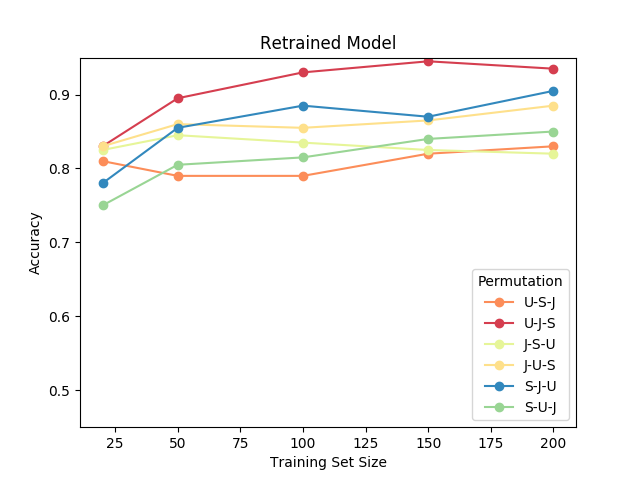
\includegraphics[width=1\textwidth]{images/validation-plot.png}}
  \end{center}
  \label{fig:validaton-plot}
  \caption{Results of our experiment. As we expected, the graph shows a positive correlation between the accuracy and the number of training samples.}
\end{figure}


\subsection{Computer vision versus convolutional neural networks}

\begin{figure}[h]
  \begin{center}
    \subfigure{\label{fig:tsne}\fbox{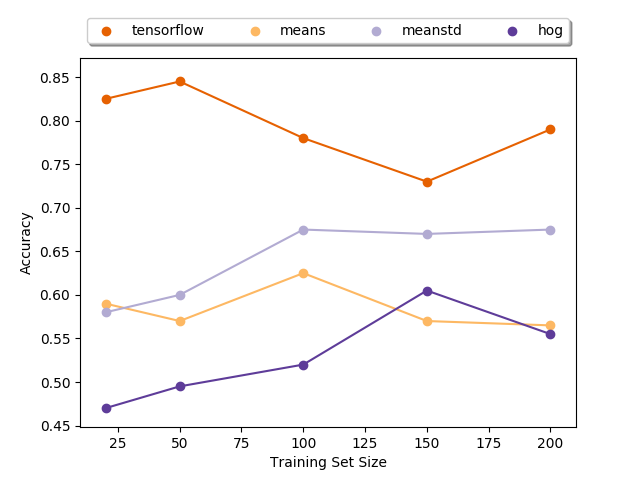
\includegraphics[width=1\textwidth]{images/accuracies-12-3.png}}}
  \end{center}
\end{figure}

\begin{figure}[h]
  \begin{center}
    \subfigure{\label{fig:tsne}\fbox{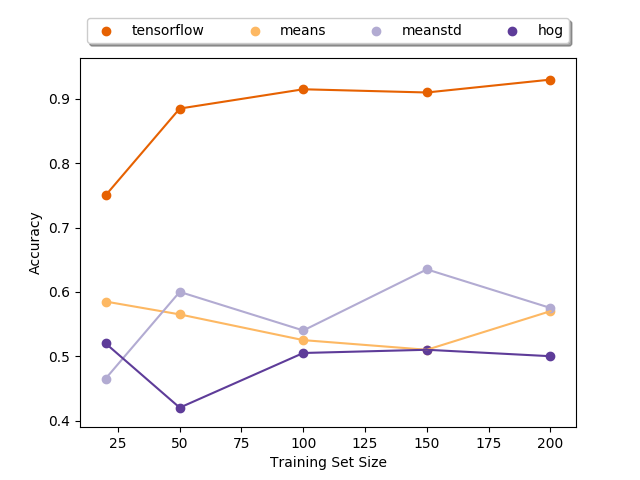
\includegraphics[width=1\textwidth]{images/accuracies-13-2.png}}}
  \end{center}
\end{figure}

\begin{figure}[h]
  \begin{center}
    \subfigure{\label{fig:tsne}\fbox{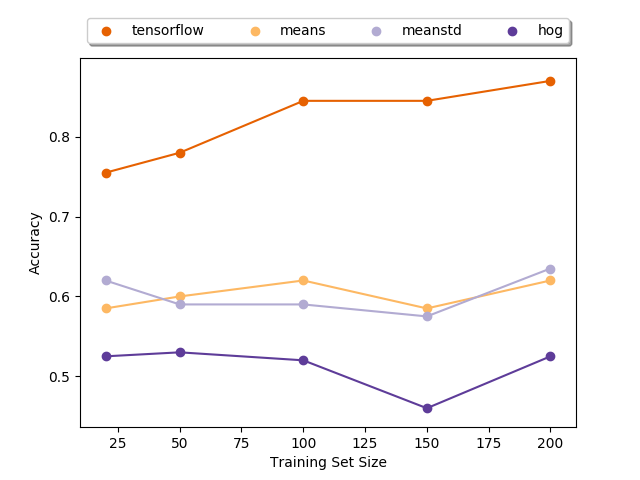
\includegraphics[width=1\textwidth]{images/accuracies-23-1.png}}}
  \end{center}
\end{figure}


\section{Threshold selection}

The binary classifier assigns a real number in the interval $[0,1]$. To decide which values will be assigined with either level a threshold must be chosen. This was picked using a ROC curve. The ROC curve helps us chosing the performance that fits our needs in the ver possible way. In order to do this we use a receiver operating characteristic curve. This tool is often used with binary classifiers to analyse the tradeoff between the true possitive rate and the false possitive rate by selecting different desicion thresholds.

\begin{figure}[h]
  \begin{center}
    \subfigure{\label{fig:tsne}\fbox{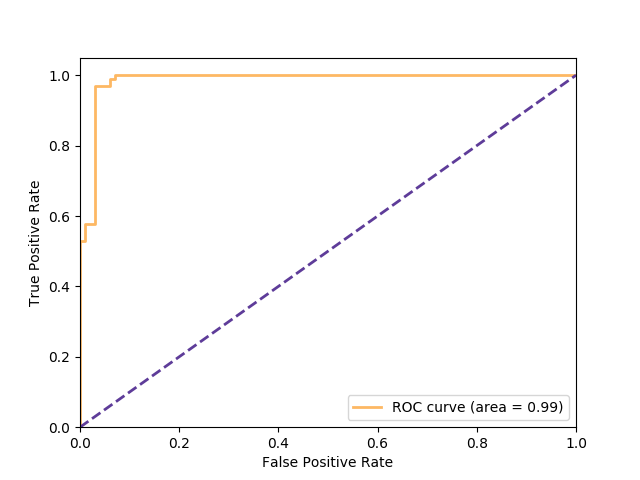
\includegraphics[width=1\textwidth]{images/roc.png}}}
  \end{center}
\end{figure}

The threshold was chosen to keep the false positive rate to 0 percent on the training set while having the highest level of true positive rate. This was atained at the following level:

\begin{center}
  \begin{tabular}{|c|c|c|}
    \hline
    threshold & true positive rate & false positive rate \\ \hline
    0.983629 & 0.529412 & 0.0 \\
    \hline
  \end{tabular}
\end{center}

The reason behind this decision was the high number of false positives shown in preliminary experiments. We want only to look at places in which the model is very confident of finding a damaged building. This theshold can be tunned to match the desired behavior in the requiered application.

\section{Results}

Ortorectified mosaics where built by CENAPRED using the very same images taht we used to train our models. This images come in a different format than the images taken by the drones. Additional to the optical information these tif files contain geographical location and can be used to assing a point in space to each pixel in the image. This means that we can not only locate a damaged building in an image, but to link this information with a geographical location in a given projection.\\

The images where divided in a regular grid of 299 pixel tiles with 90 pixel ovelaps. These overlaps are later postprocessed to eliminate the posibility of counting the same building twice. Each tile is exposed to the model which predicts a class on it using the previously selected threshold. When the model test a tile positive, the box is saved for postprocesing in which a technique known as non max suppression is used to eliminate boxes that represent the same object. This technique is borrowed from facial recognition algorithms. Once we have the final boxes, the center pixel of each box is transformed to world coordinates. Additionaly, this coordinates are used to query Google Maps API to obtain a human readable address for each point.


\begin{center}
  \begin{tabular}{|c|c|c|c|c|c|}
    \hline
    town                 & positives & width & height & time (seconds) & overlap\\ \hline
    Santa Maria Xadani   &51         & 25598 & 30144  & 4420           & 0.1 \\ \hline
    Juchitan de Zaragoza &302        & 42375 & 28831  & 6375           & 0.1 \\ \hline
    Union Hidalgo        &25         & 19945 & 28795  & 3938           & 0.1\\
    \hline
  \end{tabular}
\end{center}

A shape file is produced which contains the results for each town given the output of the algorithm. This shape can be overlayed on top of the raster file using a Geographic Information System software such as QGIS. Additionaly the results are also exposed via the REST interface so they can be visualised in the web application.



